\section{The Visual Analytics System}\looseness=-1
\label{section:design}

%To enable exploration of event sequence data, we present an interactive visual analytics system implemented in a prototype web application. Fig.~\ref{fig:teaser} shows the graphical user interface. In this section, we first introduce the analytic tasks. Then we describe the visual designs and the user interactions. 

\subsection{Analysis Tasks}\looseness=-1

In a recent paper, Plaisant and Shneiderman \cite{plaisant2016tasks} summarize a set of high-level analytic tasks for event sequence data. To identify the most common tasks across various application domains in order to design a generic tool for event sequence analysis,  we survey design studies for different kinds of data (e.g., website click streams and EHR data) and gather requirements from experts in vehicle data analytics, the new application domain we introduce in this paper. Table. 1 (Appendix) summarizes the result of the survey and the expert interview. We conclude the four high level tasks \textit{\textbf{T1, T2, T5, T7}} to be the most common ones and centered our design around these tasks. The four tasks are:\looseness=-1
\begin{compactitem}[]
	\item \textbf{\textit{T1}}. Review in detail a few records.
	\item \textbf{\textit{T2}}. Compile descriptive information about the dataset or a subgroup of records and events (esp. through aggregated views).
	\item \textbf{\textit{T5}}. Identify a set of records of interest.
	\item \textbf{\textit{T7}}. Study antecedents or sequelae of an event of interest.
\end{compactitem}

We design the system to support the aforementioned tasks while following the general guideline of showing multiple levels of detail \cite{shneiderman1996eyes}. Starting from an overview of the sequential patterns (\textbf{\textit{T2}}), the analyst can identify a subset for further investigation (\textbf{\textit{T1}}). The analyst can also filter records by their attribute values or filter events by their co-occurrences (\textbf{\textit{T1}}, \textbf{\textit{T2}}, \textbf{\textit{T5}}). The system also supports interactive alignment on a selected event to study its causes and effects (\textbf{\textit{T7}}).\looseness=-1

\subsection{Event Filter}\looseness=-1

The event filter (Fig.~\ref{fig:teaser} (C)) shows the events' co-occurrences in the sequences and allows users to select a few highly interdependent ones for further study. Similar to the design by Chuang et al. \cite{Chuang2012}, we show explicitly the co-occurrence of all the events with a focus event in the visualization. The co-occurrence is measured by Jaccard Index and is encoded as the radial distances to the focus event at the center of the display. The analyst can change the focus interactively and the distances will change accordingly. The sizes of the circles represent how frequent the events occur overall. The events are arranged around the circle based on their category. \revision{The radial angles separate different categories of events as in \cite{Chuang2012}. The categorical labels are displayed along the sectors.} \looseness=-1

The color of the cirle encode the type of the event. Using color to encode event type is a common practice in event sequence visualization \cite{monroe2013temporal, liu2017patterns}. It is also proved as relatively effective in a recent study \cite{ruddle2016methods}. The color encoding is shared across multiple views for consistency. \looseness=-1

In the visualization, events that frequently co-occur with the focus event are close to the center. The analyst can use a lasso tool to select a set of highly relevant events and focus on the sequential patterns containing those events.\looseness=-1

An alternative way to visualize the events' interdependency is Multidimensional Scaling(MDS), which can project the events to a 2D plane based on their co-occurrences. We use the radial design to show \textit{undistorted} distances to a \textit{focus} event. \revision{By observing the radial distance to the center, users can easily estimate the frequency of co-occurrence between any event and the focus event. Compared with the MDS layout, it can display more accurate and interpretable information to the analysts. Besides that, the radial layout is also suitable when the analyst wants to focus on a particular type of event.}\looseness=-1

\subsection{Summary View}\looseness=-1

In the summary view (Fig.~\ref{fig:teaser} (A)), we vertically list all the sequential patterns identified by the algorithm. Each pattern represents a cluster of sequences. For each pattern, we layout the events from left to right and display them as rectangles. The color of the rectangles encodes the type of the event. \looseness=-1

Besides displaying the sequentially ordered events in the patterns, the summary view also shows the number of edits in the corrections part. Fig.~\ref{fig:mdl_representation} illustrates the visual encoding in the summary view. Triangular glyphs are placed between adjacent events or at the beginning/end of the pattern. Their sizes are proportional to the number of insertions at the corresponding position, accumulated over all the sequences in the cluster. The height of the rectangles is proportional to the number of sequences containing the corresponding event in the pattern. It implicitly shows the deletions as the `missing' parts compared to the others. The event insertions and deletions are obtained by backtracking the dynamic programming algorithm which computes the minimum editing distances between the individual sequences and the patterns.\looseness=-1
%Swapping the positions of adjacent events can also be encoded in a similar manner by showing the accumulated number of changes in the rectangles. 

The design itself is simple in the sense that at most $O(\sum_{(P, G) \in \mathscr{C}}len(P))$ visual elements appears in it (counting the rectangles and triangles). It is a \textit{lossy} representation of the original data since detailed information of each edit is missing and it is not possible to recover all the original sequences with this visual representation. The sizes of the triangles and the heights of the rectangles visually indicate the amount of information loss. This design also helps viewers identify clusters with high/low intra-cluster similarity, which can guide them to a more detailed exploration of the data. For example, Fig.~\ref{fig:teaser} (A.0 $\rightarrow$ A.1) shows how the user can expand a triangle and get a summary view of the subsequences in it. \revision{One potential drawback of this design is that missing events are not explicitly encoded. In certain application scenarios (e.g. EHR data analysis), missing events may also need to be highlighted with additional visual cues.}\looseness=-1

%\begin{figure}[h]
%	\centering
%	\includegraphics[width=0.95\linewidth]{pictures/summary_view}
%	\caption{A visual summary of the six sequences in Fig.~\ref{fig:mdl_representation} using the two sequential patterns. The height of the rectangles is proportional to the number of sequences containing the corresponding event. Triangular glyphs encode the number of event insertions. Note that this is a \textit{lossy} representation of the original data: it is not possible to recover the original sequences without detailed information about each edit. The size of the triangle glyphs and the height of the rectangles visually indicate the amount of information loss.}
%	\label{fig:summary_view}
%\end{figure}

\subsection{Sequence View}\looseness=-1

The sequence view (Fig.~\ref{fig:teaser} (B)) organizes the detailed information of each record in a tabular form. The attribute values and the original event sequences are displayed. The events are placed along a horizontal axis. Each event is represented by a glyph. The events matched in the patterns are displayed in larger sizes. Event sequences in the same cluster are placed together.\looseness=-1

\subsection{User Interaction}

\revision{User interactions are designed to support the exploration of event sequence data. We summarize the interactions into three categories.}\looseness=-1

\revision{\textbf{Basic interactions.} Filtering, tooltip and linked-highlighting are the three basic interactions supported in our system. The system support two types of filtering. First, as mentioned in Section 5.2, users can filter events with the lasso selection tool in the event filter (Fig.~\ref{fig:teaser} (C)). The analysts can also filter the sequences through the attribute values as shown in Fig.~\ref{fig:teaser} (D). Note that the event filter will always be updated accordingly to reflect the co-occurrences of events in the filtered sequences in Fig.~\ref{fig:teaser} (D). The filtering function is especially helpful when the analysts have prior knowledge about what kind of sequences or events worth further analysis. A tooltip is designed to show the detailed description of each event when analysts hover over any event in the system. Furthermore, linked-highlighting is supported to help users associate the information displayed in the detailed view (Fig.~\ref{fig:teaser} (B)) with the summary view (Fig.~\ref{fig:teaser} (A)). When users click and highlight patterns in the summary view, individual sequences in the detailed view will be ordered and highlighted accordingly.}\looseness=-1

\revision{\textbf{Detail on demand.} As mentioned in Section 5.3, inserted events are aggregated and visualized as triangular glyphs in the summary view. However, users may still want to examine the details, especially when the size of the glyphs indicate that there are many inserted events. In the prototype, the users can double click the glyphs to expand them for detailed analysis. To be more specific, since the inserted events are also a set of subsequences, we apply the same summarization approach in Section 4 to these subsequences and show a set of patterns and corrections in the expanded view. Fig.~\ref{fig:teaser} (A.0 $\rightarrow$ A.1) shows an example of such expansion.}\looseness=-1

\revision{\textbf{Temporal relation exploration.} To support efficient temporal relation exploration, we allow users to align sequences at a selected event. By default, the sequences in summary view and the detail view are aligned at the first event. Users can select one event in the summary view and both views will be aligned to the selected event through animated transition. Fig.~\ref{fig:teaser} (A, B) shows an example where the events are aligned at the event `gh'. In this way, users can easily identify subsequences occur before and after a given event. Besides, the horizontal scale in the detailed view can be changed to show accurate temporal information instead of only sequential orders. By changing the scale, the users can analyze the temporal distribution of events. Users can also combine alignment and changing the horizontal scale in the system. In this way, they can easily observe the how other events distribute with respect to a selected event. Fig.~\ref{fig:case0_1} shows an example.}\looseness=-1

\revision{The system also has other interactive features such as reordering the patterns in the summary view. The analyst can sort the sequential patterns by 1) the number of sequences in the corresponding cluster and 2) the similarity between the patterns measured through the editing distance. To reorder by similarity, we first perform a hierarchical clustering of the patterns and then sort them by the leaf order.}\looseness=-1

\begin{figure}[h]
	\centering
	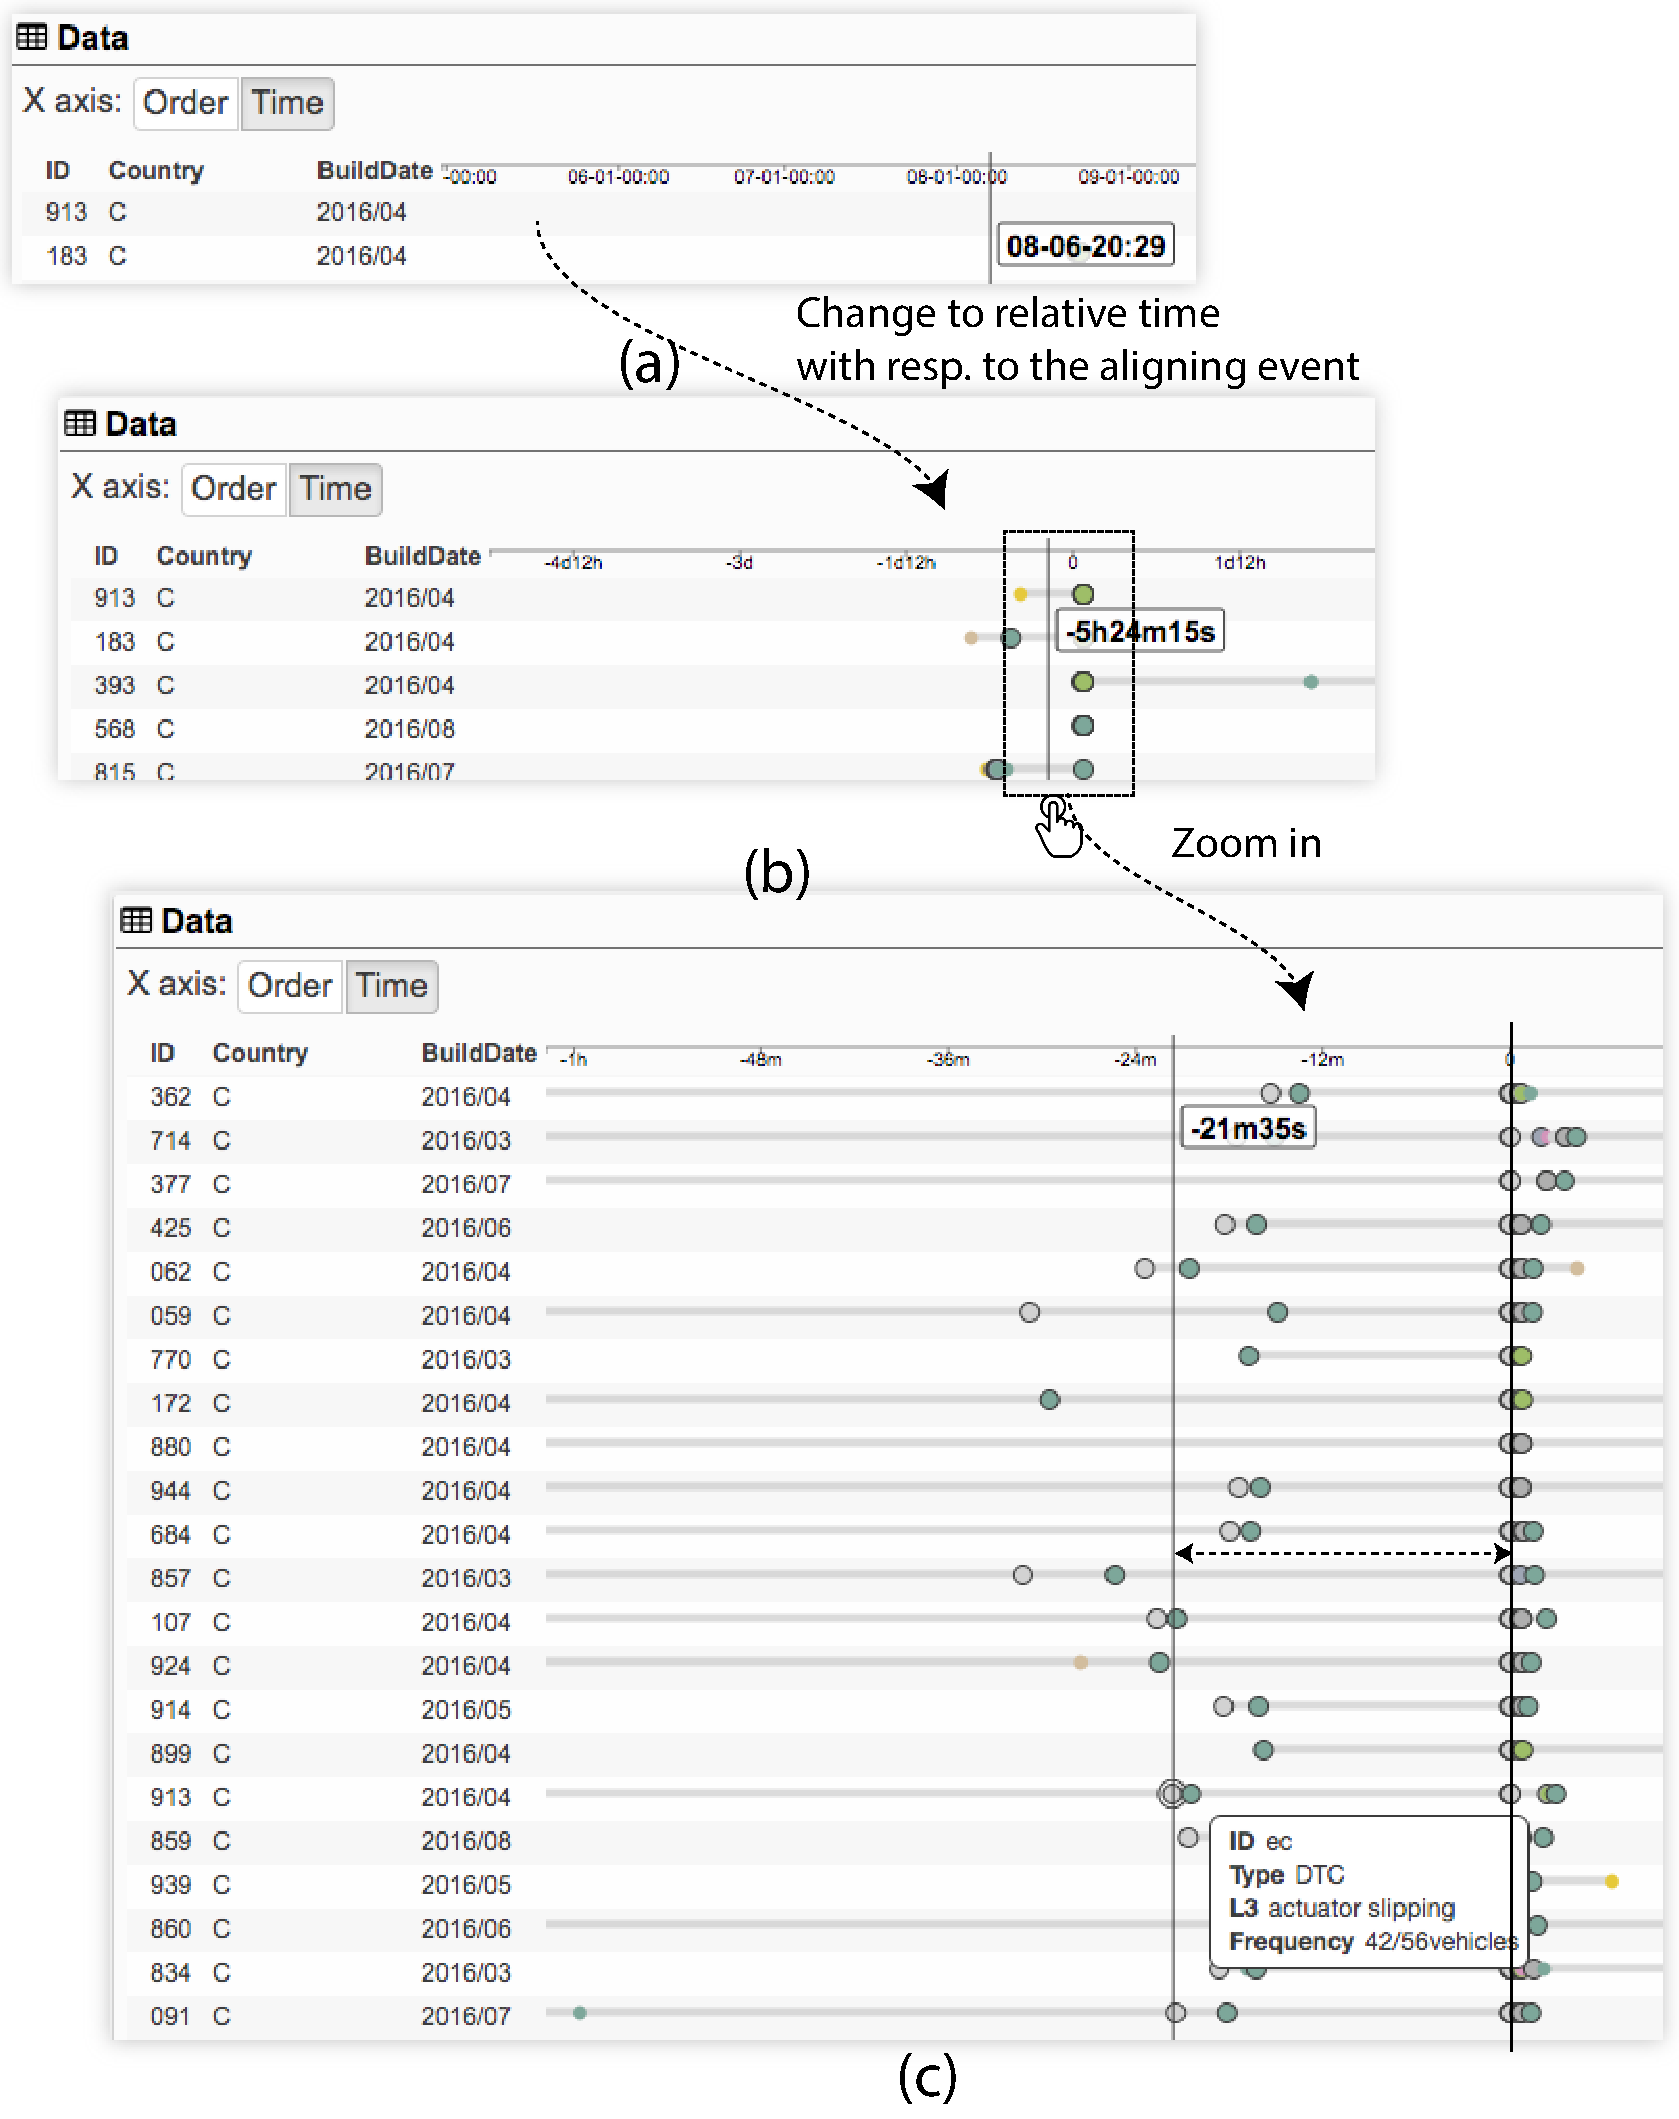
\includegraphics[width=0.96\linewidth]{pictures/case3}
	\caption{Switching X axis to timestamps. (a) by default absolute time is displayed (b) aligning at an event changes the X axis to relative time (c) zooming in on the timeline shows that most events in the pattern occurred within a 20 minutes time range. %indicating a causal relationship that took place pretty fast.
		 \looseness=-1}
	\label{fig:case0_1}
\end{figure}

%\subsection{Implementation}
%
%We implement the system as a web application. The front-end visualization is implemented with D3\footnote{https://d3js.org/} and several JavaScript libraries include BackBone.js\footnote{http://backbonejs.org/} and Underscore.js\footnote{http://underscorejs.org/}. The back-end is implemented in Python with the Flask\footnote{http://flask.pocoo.org/} web application framework and we use the weighted LSH algorithm implemented in the datasketch\footnote{https://github.com/ekzhu/datasketch/} library.